% ================================================================
% chapters/chapter5.tex --- RECONSTRUCTION (même structure que ch.3)
% ----------------------------------------------------------------
% Backlog restructuré~: Titre + Charge (j/h) ajoutées, Statut retiré
% + phrase de synthèse. Charge (j/h) = MES ESTIMATIONS RELATIVES,
% pas des mesures réelles --- à remplacer si tu as de vraies données.
% Rien d'autre n'est modifié dans ce chapitre.
% ================================================================

\chapter{Itération~3 --- Application VR Meta Quest~3 (scènes d'authentification)}

\section{Introduction}

 Cette itération couvre le développement de l'application VR pour Meta Quest~3, incluant
les deux premières scènes~: la scène tutoriel (\texttt{trainingscene}, initiation aux contrôleurs) et
la scène d'authentification (\texttt{Companys}, connexion et sélection des formations). À l'issue de cette itération,
un employé peut activer le casque, se connecter, voir les formations disponibles
et accéder aux paramètres.

\section{Planification de l'itération~3}

Cette section définit les objectifs de la troisième itération, les tâches associées et
leur charge estimée.

\subsection{Objectifs}

\begin{itemize}
  \item Implémenter le flow complet d'activation du casque (Meta User ID matériel + code d'activation à 6 chiffres).
  \item Permettre le login employé (accessCode + PIN) via une interface VR intuitive.
  \item Charger et afficher les formations assignées à l'entreprise.
  \item Livrer un tutoriel d'introduction aux contrôleurs Meta Quest~3.
  \item Permettre la configuration des paramètres (audio, langue, contrôleurs).
\end{itemize}

\subsection{Tâches et estimations de l'itération~3}

\begin{table}[H]
  \centering
  \small
  \setlength{\tabcolsep}{5pt}
  \begin{tabularx}{\textwidth}{cp{3.5cm}Xc>{\footnotesize}c}
    \toprule
    \textbf{ID} & \textbf{Titre} & \textbf{Description} & \textbf{MoSCoW} & \textbf{Charge (j/h)} \\
    \midrule
    US-14 & Tutoriel des contrôleurs &
      Scène tutoriel (\texttt{trainingscene}) --- 3 leçons & \must{} & 4 \\
    US-15 & Activation du casque &
      DeviceActivationManager (Meta User ID + code d'activation) & \must{} & 2 \\
    US-16 & Connexion employé &
      EmployeeSignInPanel (code + PIN numpad) & \must{} & 3 \\
    US-17 & Liste des formations &
      ModulesPanel (grille formations) & \must{} & 2,5 \\
    US-18 & Paramètres persistants &
      SettingsPanel (audio, langue, contrôleurs) & \should{} & 3 \\
    \midrule
    \multicolumn{4}{r}{\textbf{Total estimé}} & \textbf{14,5} \\
    \bottomrule
  \end{tabularx}
  \caption{Tâches et estimations --- Itération~3}
  \label{tab:backlog_s3}
\end{table}

\noindent Toutes les user stories de cette itération ont été livrées.

\section{Conception de l'itération~3}

Cette section présente la configuration du projet Unity pour Meta Quest~3, les décisions
architecturales de l'application et l'organisation de ses scripts principaux.

\subsection{Configuration Unity~6 pour Meta Quest~3}

\begin{table}[H]
  \centering
  \begin{tabularx}{\textwidth}{lX}
    \toprule
    \textbf{Paramètre} & \textbf{Valeur} \\
    \midrule
    Plateforme cible     & Android (ARM64) \\
    API graphique        & Vulkan (recommandé Quest~3) \\
    XR Plugin            & Meta OpenXR \\
    Features activées    & Meta Quest Support, Foveated Rendering,
                           Hand Interaction Poses, XR Performance Settings \\
    Profils contrôleurs  & Meta Quest Touch Plus, Meta Quest Touch Pro \\
    Niveau API minimum   & Android 10 (API 29) \\
    \bottomrule
  \end{tabularx}
  \caption{Configuration Unity~6 pour Meta Quest~3}
  \label{tab:unity_config}
\end{table}

\subsection{Décisions architecturales --- Unity}

\begin{table}[H]
  \centering
  \begin{tabularx}{\textwidth}{lllX}
    \toprule
    \textbf{Composant} & \textbf{Retenu} & \textbf{Alternative} & \textbf{Justification} \\
    \midrule
    Moteur & Unity 6 LTS & Unreal Engine 5 & 85\% des apps Quest Store en 2024,
                                             Meta XR SDK optimisé Unity \\
    SDK    & Meta XR All-in-One & Meta Core SDK & Un seul package intégrant tous les
                                                  SDK Meta \\
    Client HTTP & TynassApiClient & ApiManager (obsolète) & Singleton avec JWT,
                                                              méthodes typées, PlayerPrefs \\
    État global & AppSession & SessionManager & Classe statique~: toujours disponible
                                                sans instanciation, pas de cycle de vie \\
    \bottomrule
  \end{tabularx}
  \caption{Décisions architecturales --- Unity}
  \label{tab:archi_unity}
\end{table}

\begin{archbox}
  \textbf{AppSession vs SessionManager}~: \texttt{SessionManager.cs} en tant que
  MonoBehaviour singleton nécessite un GameObject dans la scène et dépend du cycle
  de vie Unity. \texttt{AppSession.cs} est une classe statique C\# toujours disponible
  sans instanciation, sans \texttt{DontDestroyOnLoad}, sans risque de destruction
  entre scènes. Pour des données d'état global (token, employé connecté, formation
  active), la classe statique est architecturalement plus appropriée.
\end{archbox}

\subsection{Architecture Unity --- Scripts principaux}

L'application Unity s'organise autour de huit scripts principaux, regroupés par
responsabilité~: communication avec le backend, gestion de l'état global, navigation
entre les interfaces, et activation du casque. La figure~\ref{fig:composants_unity}
présente ces composants et leurs dépendances.

\begin{figure}[H]
  \centering
  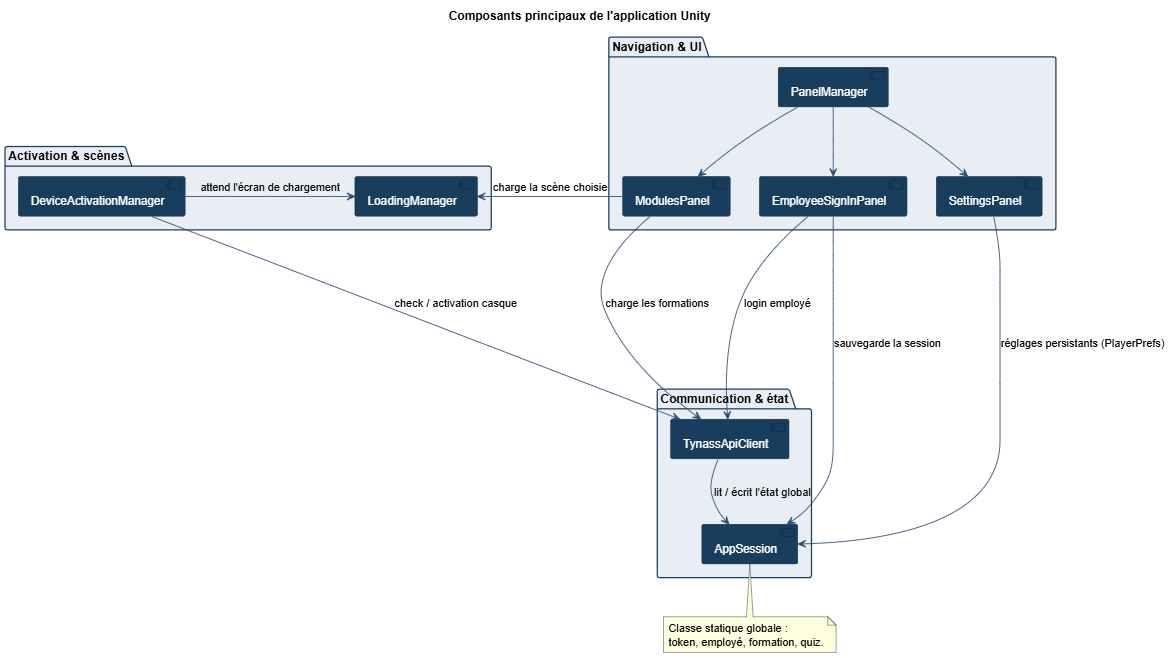
\includegraphics[width=\textwidth]{../images/composantsUnity.png}
  \caption{Diagramme de composants des scripts principaux de l'application Unity}
  \label{fig:composants_unity}
\end{figure}

Les 8 scripts principaux de l'application Unity~:

\begin{itemize}
  \item \textbf{TynassApiClient.cs}~: singleton HTTP centralisé. Gère le JWT
    (\texttt{SetToken}/\texttt{ClearToken}), \texttt{TryRestoreSession()} au
    démarrage, et toutes les méthodes typées de l'API. Utilise les classes
    \texttt{[Serializable]} pour la sérialisation JSON via \texttt{JsonUtility}.
  \item \textbf{AppSession.cs}~: classe statique globale. Stocke les données de
    Device, Company, Employee, Training et Quiz (QuizScore, QuizCorrect, QuizTotal,
    QuizCurrentIndex, QuizElapsedSecs). \texttt{AppSession.Clear()} efface les
    données personnelles de l'employé mais conserve le DeviceToken (appartient au
    casque).
  \item \textbf{PanelManager.cs}~: gère la navigation entre les panels UI
    (GoSignIn, GoEmployeePicker, GoModules, GoSettings, GoQuiz, GoQuizResult).
  \item \textbf{DeviceActivationManager.cs}~: récupère le Meta User ID via
    \texttt{Oculus.Platform.Users.GetLoggedInUser()}, orchestre le flow
    d'activation.
  \item \textbf{EmployeeSignInPanel.cs}~: gère les 2 étapes de login (Step~1~:
    accessCode XX-001, Step~2~: PIN numpad 4 chiffres).
  \item \textbf{ModulesPanel.cs}~: charge les formations via \texttt{device\_token},
    instancie les cartes de formation dans un Grid Layout Group.
  \item \textbf{SettingsPanel.cs}~: audio (master/sfx/narration/spatial), langue
    (FR/EN/AR), contrôleurs (main, dwell time, haptic). Persistance via
    \texttt{PlayerPrefs}.
  \item \textbf{TrainingSceneManager.cs}~: orchestre la scène tutoriel
    (\texttt{trainingscene})~: leçons, narration audio, NarrationManager.
\end{itemize}

\subsection{Cas d'utilisation --- Descriptions textuelles}

\begin{ucbox}{Tutoriel d'introduction (scène \texttt{trainingscene})}
  \begin{tabular}{lp{9cm}}
    \textbf{Pré-conditions} & Casque démarré, utilisateur novice en VR. \\
    \textbf{Acteur}         & Employé. \\
    \textbf{Scénario A}     &
      1. L'utilisateur choisit « Commencer les leçons » (choix A). \newline
      2. Leçon 1~: se déplacer avec le joystick jusqu'au waypoint. \newline
      3. Leçon 2~: saisir un cube (grip) et l'amener au waypoint. \newline
      4. Leçon 3~: lire un panel, cliquer sur le bouton (trigger). \newline
      5. Transition automatique vers la scène Companys. \\
    \textbf{Scénario B}     &
      1. L'utilisateur choisit « Passer » (choix B). \newline
      2. Transition directe vers la scène Companys. \\
    \textbf{Post-conditions}& Utilisateur maîtrise les 3 interactions fondamentales. \\
  \end{tabular}
\end{ucbox}

\vspace{0.5cm}

\begin{ucbox}{Sélectionner une formation (ModulesPanel)}
  \begin{tabular}{lp{9cm}}
    \textbf{Pré-conditions} & Employé connecté, \texttt{device\_token} valide. \\
    \textbf{Acteur}         & Employé. \\
    \textbf{Scénario}       &
      1. ModulesPanel appelle \texttt{GET /api/company/devices/trainings}. \newline
      2. Les formations assignées à l'entreprise sont affichées en grille. \newline
      3. L'employé pointe et sélectionne une formation. \newline
      4. \texttt{AppSession.ActiveTraining} est défini. \newline
      5. \texttt{SceneManager.LoadScene(training.sceneName)} est appelé. \newline
      6. Si \texttt{sceneName} est null~: erreur loguée, rien ne se passe. \\
    \textbf{Post-conditions}& Scène de formation chargée. \\
  \end{tabular}
\end{ucbox}

\subsection{Diagramme de séquence}

La figure~\ref{fig:flow_complet} retrace le flux complet vécu par un employé, depuis le
tutoriel jusqu'au lancement d'une simulation, en passant par l'authentification et la
sélection d'une formation. Elle montre l'enchaînement des trois scènes et leurs échanges
avec le backend.

\begin{figure}[H]
  \centering
  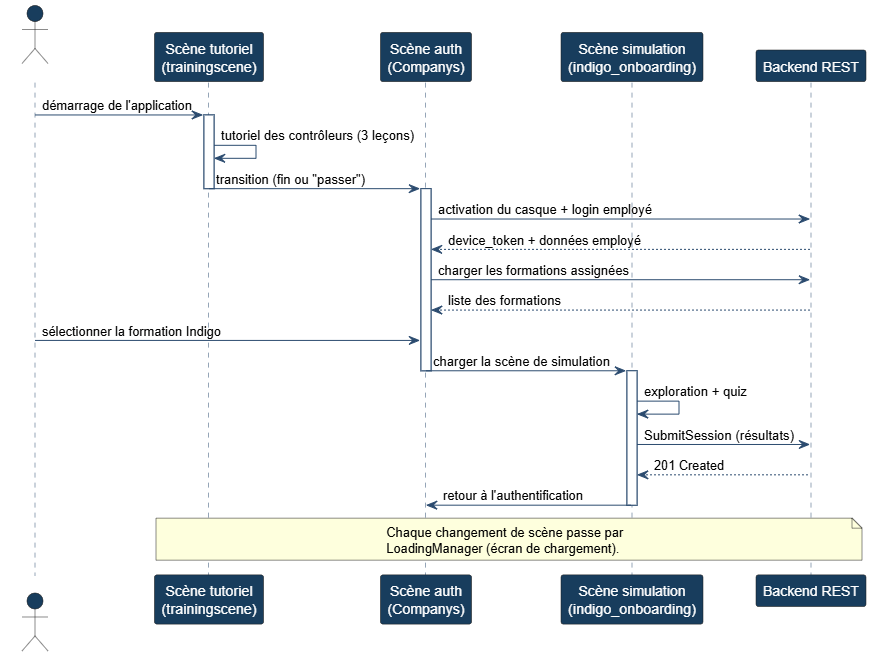
\includegraphics[width=0.9\textwidth]{../images/flowComplet.png}
  \caption{Diagramme de séquence --- flux complet entre les trois scènes}
  \label{fig:flow_complet}
\end{figure}

\section{Implémentation de l'itération~3}

Cette section détaille la mise en œuvre des principaux composants de l'application~: le
client HTTP, l'activation du casque, le login employé et les panneaux de l'interface.

\subsection{TynassApiClient.cs --- Client HTTP centralisé}

\texttt{TynassApiClient} est le singleton central de communication avec le backend.
Sa conception résout un problème fondamental de Unity~: \texttt{JsonUtility} ne
sérialise que les classes marquées \texttt{[Serializable]}. Tout objet anonyme
produit un JSON vide (\texttt{\{\}}).

 \begin{lstlisting}[language={[Sharp]C}, caption={TynassApiClient -- methode typee async}]
[Serializable]
public class EmployeeLoginPayload {
    public string accessCode;
    public string pin;
}

public async Task<EmployeeLoginResponse> LoginEmployee(
    string accessCode, string pin, string deviceToken)
{
    var payload = new EmployeeLoginPayload { accessCode = accessCode, pin = pin };
    // POST /company/employees/login avec le device_token dans l'en-tete
    return await PostRequest<EmployeeLoginResponse>(
        "/company/employees/login", payload, deviceToken);
}
\end{lstlisting}

\subsection{DeviceActivationManager --- Meta User ID}

\begin{lstlisting}[language={[Sharp]C}, caption={Meta User ID -- recuperation et verification}]
Oculus.Platform.Users.GetLoggedInUser().OnComplete(async msg => {
    string metaUserId;
    if (!msg.IsError)
        metaUserId = msg.Data.ID.ToString();
    else
        metaUserId = SystemInfo.deviceUniqueIdentifier; // fallback editeur

    var response = await TynassApiClient.Instance.CheckDevice(metaUserId);
    if (response != null && response.status == "activated")
        ShowLoginPanel();
    else
        ShowActivationPanel();
});
\end{lstlisting}

\subsection{EmployeeSignInPanel --- Login en 2 étapes}

\begin{enumerate}
  \item \textbf{Step 1 --- accessCode}~: l'employé saisit son code via un clavier
    alphanumérique. Unity valide le format en temps réel avec
    \texttt{Regex.IsMatch(code, \^{}[A-Z]\{2\}-\textbackslash d\{3\}\$)}.
    Cette validation côté Unity donne un retour immédiat sans aller-retour réseau.
    La validation backend constitue la sécurité réelle (défense en profondeur).
  \item \textbf{Step 2 --- PIN}~: numpad 4 chiffres (0-9 + effacer). Visuellement
    masqué par des étoiles. Envoyé au backend pour vérification bcrypt.
\end{enumerate}

\begin{figure}[H]
  \centering
  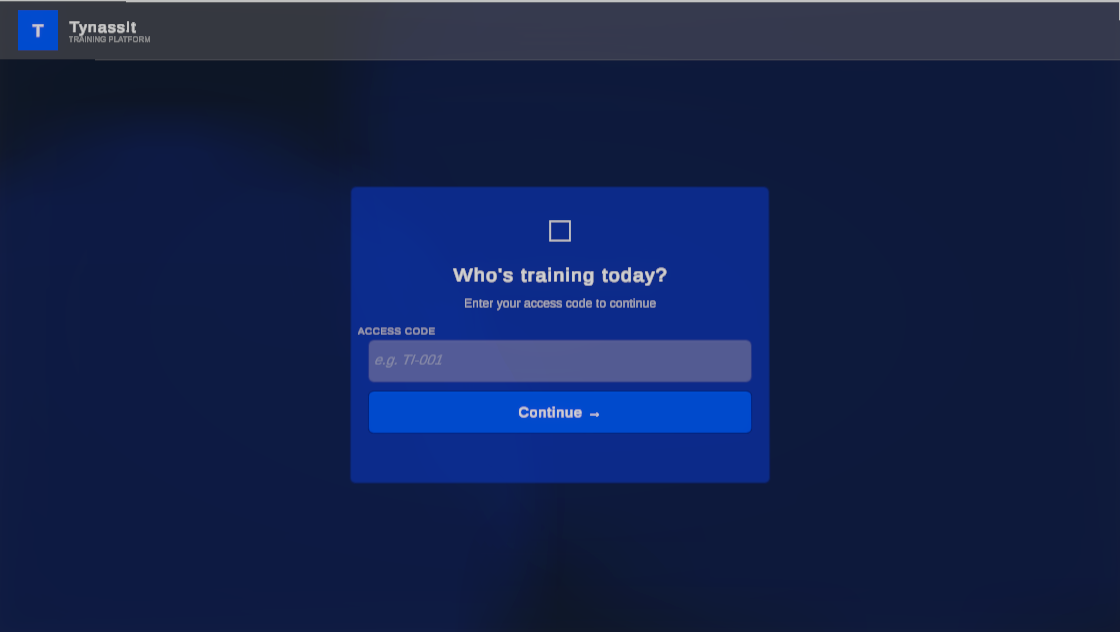
\includegraphics[width=0.7\textwidth]{../images/vr_signin_code.png}
  \caption{Connexion employé --- saisie du code d'accès}
  \label{fig:vr_signin_code}
\end{figure}

\begin{figure}[H]
  \centering
  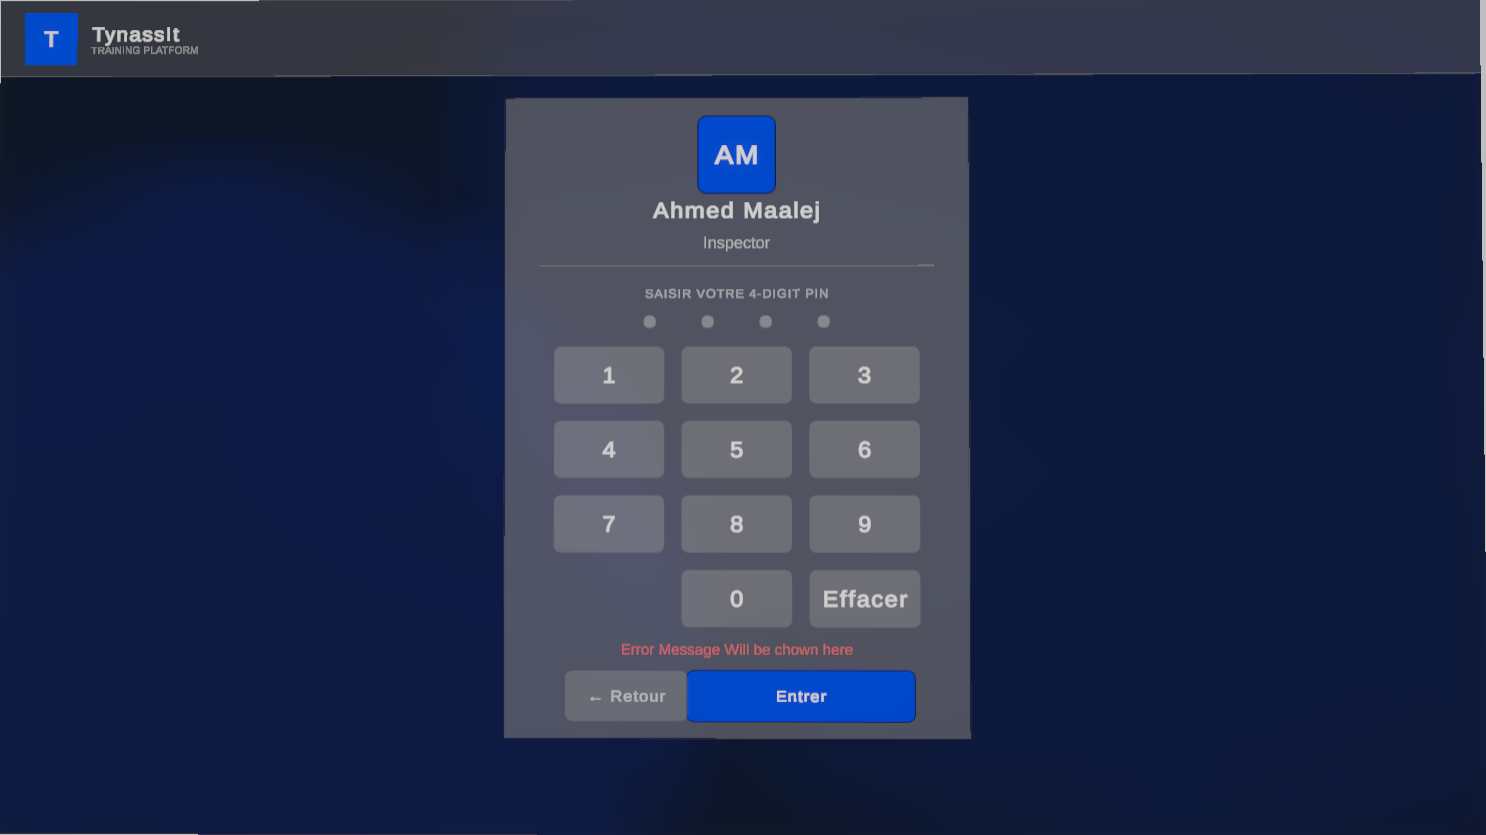
\includegraphics[width=0.7\textwidth]{../images/vr_signin_pin.png}
  \caption{Connexion employé --- saisie du PIN}
  \label{fig:vr_signin_pin}
\end{figure}

\subsection{ModulesPanel --- Grille des formations}

Les cartes de formation sont instanciées dynamiquement depuis un prefab dans un
\textbf{Grid Layout Group}, qui calcule automatiquement la position de chaque enfant
selon \texttt{Cell Size} et \texttt{Spacing}.

\begin{figure}[H]
  \centering
  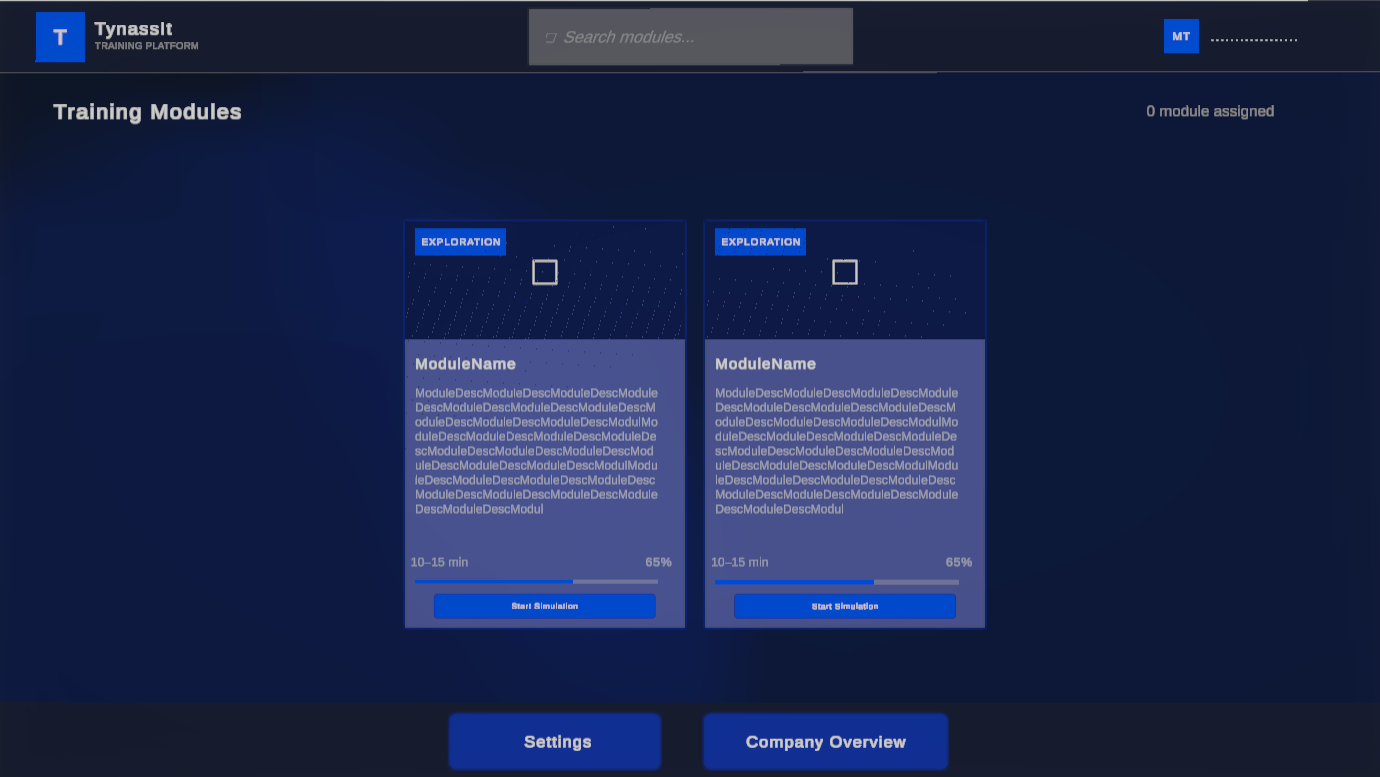
\includegraphics[width=0.8\textwidth]{../images/vr_modules.png}
  \caption{Liste des formations assignées (ModulesPanel)}
  \label{fig:vr_modules}
\end{figure}

\subsection{SettingsPanel --- Paramètres persistants}

Tous les paramètres sont sauvegardés dans \texttt{PlayerPrefs}~:
\texttt{vol\_master}, \texttt{vol\_sfx}, \texttt{vol\_narr}, \texttt{mute\_all},
\texttt{spatial}, \texttt{ui\_lang}, \texttt{narr\_lang}, \texttt{hand},
\texttt{dwell\_time}, \texttt{glow}, \texttt{haptic}.

\begin{figure}[H]
  \centering
  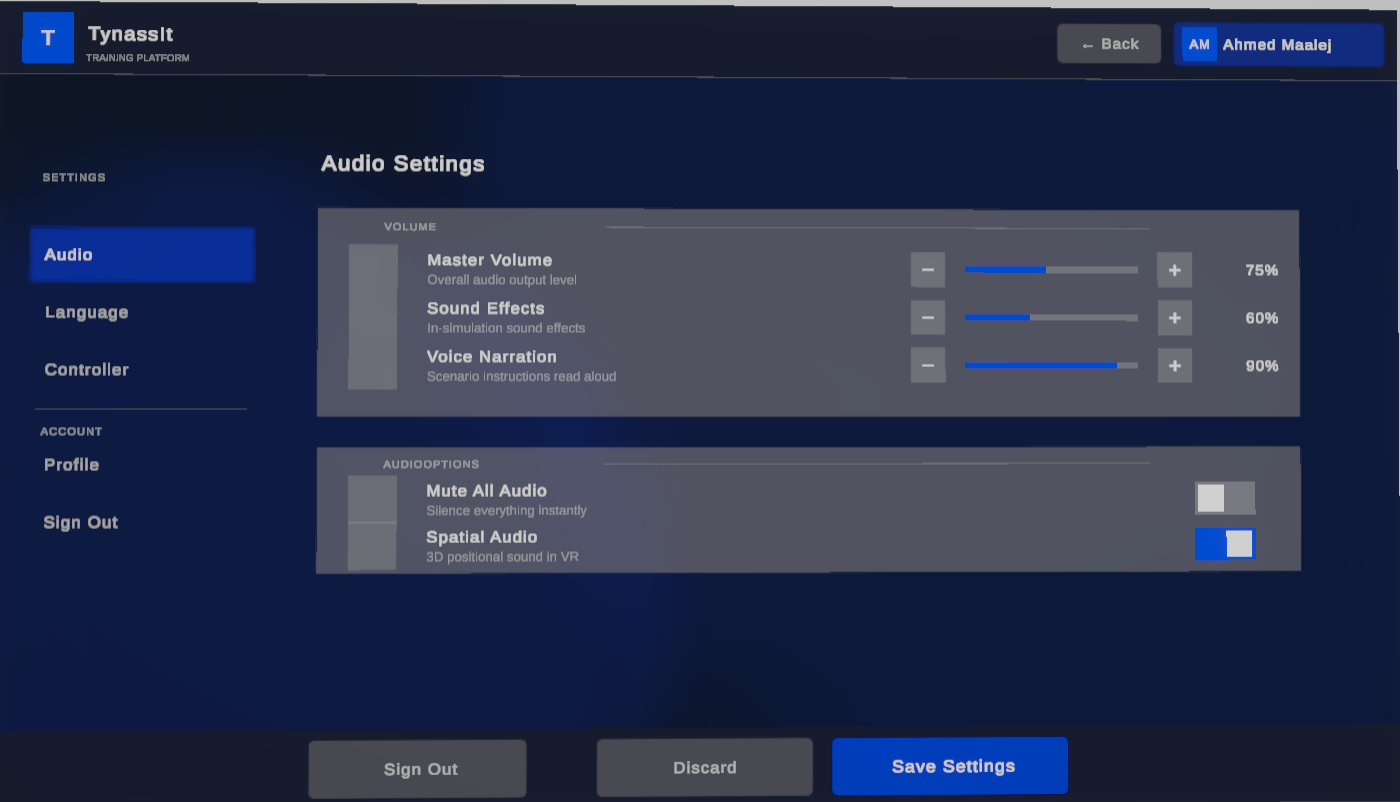
\includegraphics[width=0.8\textwidth]{../images/vr_settings.png}
  \caption{Panneau de configuration des paramètres}
  \label{fig:vr_settings}
\end{figure}

\section{Difficultés et solutions}

\begin{table}[H]
  \centering
  \begin{tabularx}{\textwidth}{lXX}
    \toprule
    \textbf{Défi} & \textbf{Problème} & \textbf{Solution} \\
    \midrule
    JsonUtility & Les objets anonymes \texttt{new \{email = "test"\}}
                  produisaient \texttt{\{\}} (JSON vide). &
                  Création de classes \texttt{[Serializable]} explicites
                  pour tous les payloads. \\
    \midrule
    Vidéos lentes & Les vidéos dans \texttt{Resources/} étaient préchargées
                    au démarrage, causant un gel de plus d'une minute. &
                    Migration vers \texttt{StreamingAssets/}~: lecture en
                    streaming via URL \texttt{file://}, démarrage instantané. \\
    \midrule
    Cards superposées & Les cartes de formations apparaissaient toutes
                        au même point (0,0,0) sans layout automatique. &
                        \texttt{Grid Layout Group} calcule automatiquement
                        la position de chaque carte. \\
    \midrule
    Vélocité locomotion & Maintenir le joystick pendant un blocage
                          accumulait une vélocité~: l'employé partait
                          en sprint au déblocage. &
                          \texttt{EnableMovement()} remet la vélocité
                          à zéro avant de réactiver le mouvement. \\
    \bottomrule
  \end{tabularx}
  \caption{Difficultés rencontrées et solutions --- Itération~3}
  \label{tab:dificultes_s3}
\end{table}

\section{Évaluation de l'itération~3}

\begin{table}[H]
  \centering
  \begin{tabularx}{\textwidth}{Xl}
    \toprule
    \textbf{Élément validé} & \textbf{Statut} \\
    \midrule
    Activation du casque sur Meta Quest~3 & Fonctionnel \\
    Login employé (code d'accès + PIN) sur le casque & Fonctionnel \\
    Affichage des formations assignées & Fonctionnel \\
    Tutoriel des contrôleurs (3 leçons) & 3 / 3 \\
    Persistance des paramètres (audio, langue, contrôleurs) & Fonctionnel \\
    \bottomrule
  \end{tabularx}
  \caption{Validation fonctionnelle --- Itération~3}
  \label{tab:eval_s3}
\end{table}

La figure~\ref{fig:vr_tuto} illustre la deuxième leçon du tutoriel, où
l'employé apprend à saisir un objet.

\begin{figure}[H]
  \centering
  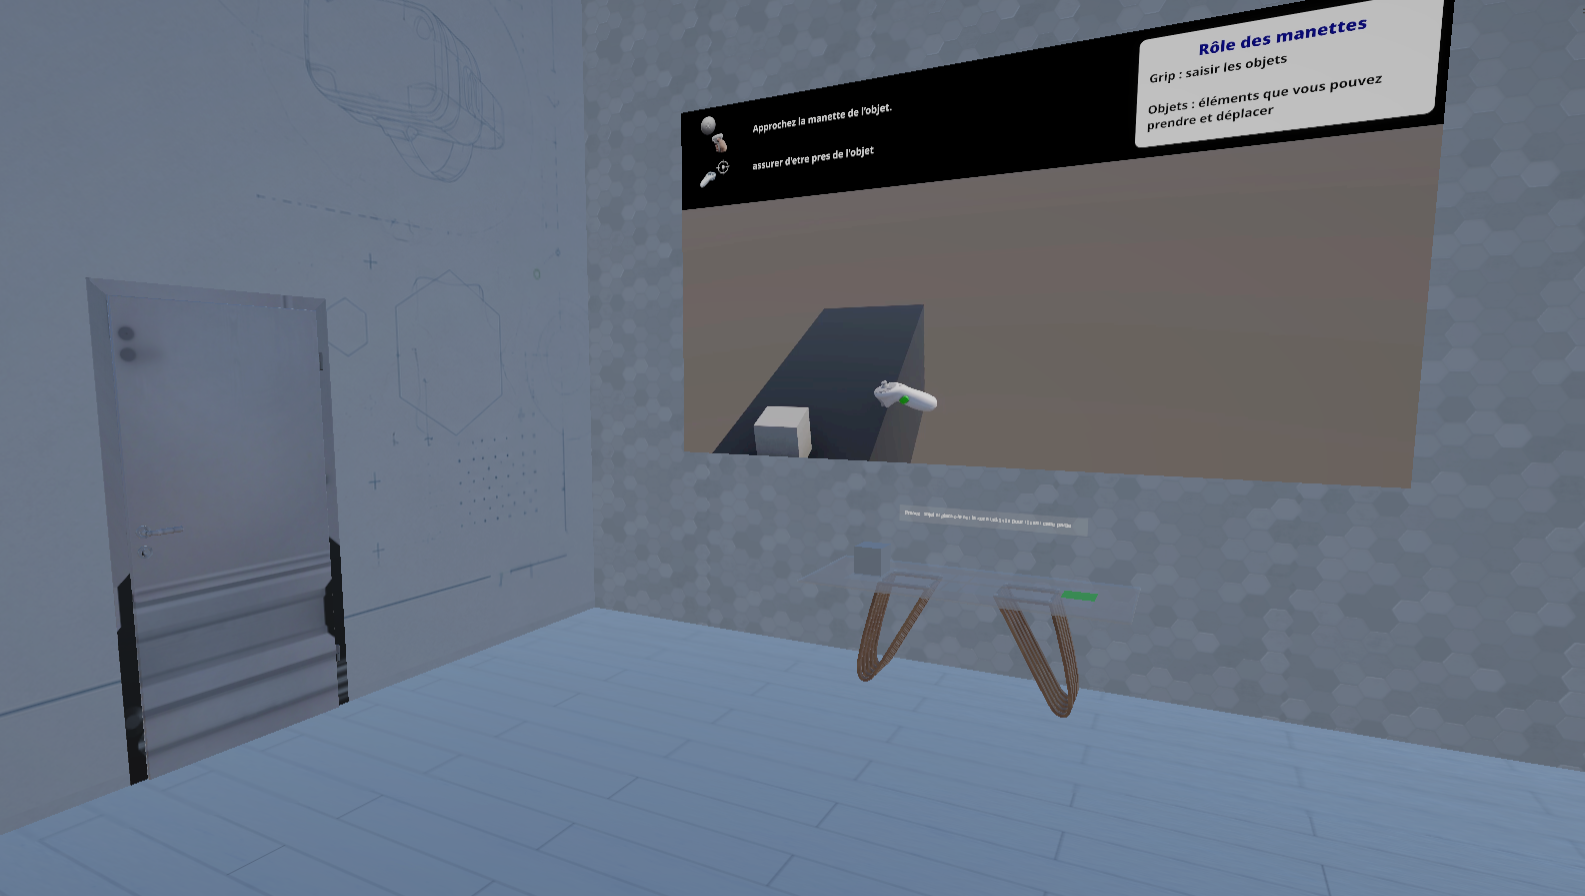
\includegraphics[width=0.8\textwidth]{../images/vr_tutoriel_grip.png}
  \caption{Scène tutoriel --- leçon de manipulation (grip)}
  \label{fig:vr_tuto}
\end{figure}

\begin{figure}[H]
  \centering
  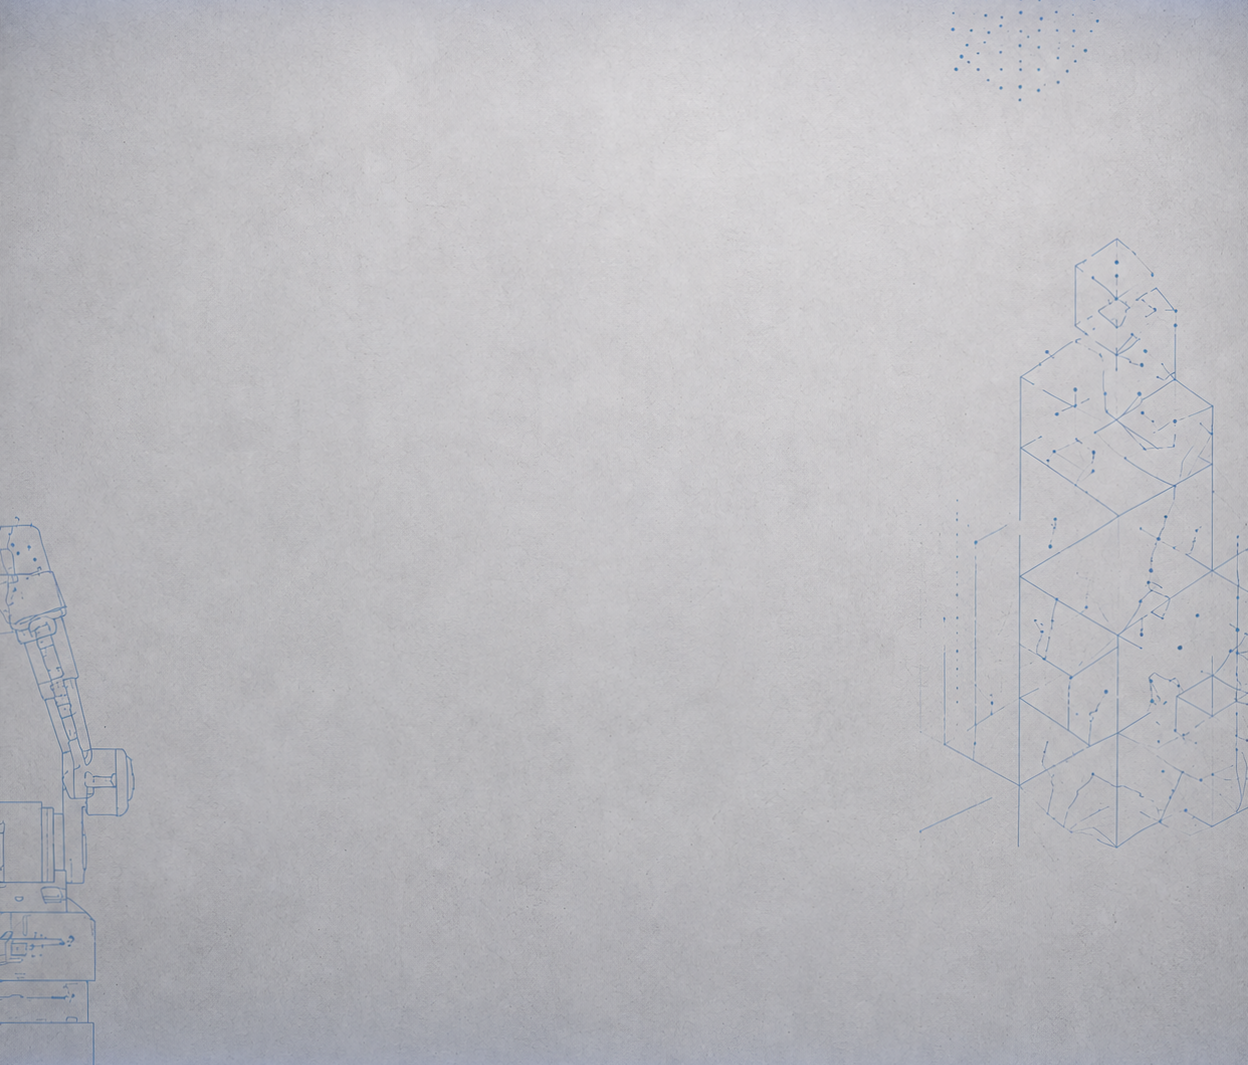
\includegraphics[width=0.9\textwidth]{../images/vr_flow_casque.png}
  \caption{Exécution du flux complet sur le casque Meta Quest~3}
  \label{fig:vr_flow_casque}
\end{figure}

\section{Conclusion}

Cette troisième itération a livré l'application VR avec ses deux premières scènes~:
le tutoriel des contrôleurs et l'authentification. Le flow complet
fonctionne sur le casque physique Meta Quest~3~: activation, login employé, affichage
des formations. Le chapitre suivant présente la simulation d'intégration d'Indigo Company.
